\documentclass[a4paper]{scrartcl}

\usepackage{hyperref} % allows linking within PDF files
\usepackage{url} % allows url references
\usepackage{fancyvrb} % for smaller, custom verbatim fonts
\usepackage[kerning,spacing]{microtype} % PDFLaTeX microtypography
\usepackage{graphicx} % enables use of graphics files other than EPS
\usepackage{fancyhdr} % does nice ``book-style'' headers / footers
\usepackage{Sweave} % for in-line R calculations
\usepackage{a4wide} % for smaller margins
\usepackage{xfrac} % for nice-looking fractions

\microtypecontext{spacing=nonfrench} % correction for microtype issue

\hypersetup{% set up link colours so that things look better when printed
    colorlinks,%
    citecolor=black,%
    filecolor=black,%
    linkcolor=black,%
    urlcolor=black
}

\begin{document}

\newcommand{\tabh}[1]{\multicolumn{1}{l}{\bfseries#1}} % for table header row

% change default figure width to fit more of the page
\setkeys{Gin}{width=0.95\textwidth}

\RecustomVerbatimEnvironment{Verbatim}{Verbatim}
{frame=single,fontsize=\scriptsize,label=ImageJ Macro}
\DefineVerbatimEnvironment{Sinput}{Verbatim}
{frame=single,fontsize=\scriptsize,label=R Script}
\DefineVerbatimEnvironment{Soutput}{Verbatim}
{frame=single,fontsize=\scriptsize,label=R Output}

% remove paragraph indentation

\setlength{\parindent}{0.0in}
\setlength{\parskip}{0.1in}


\pagestyle{fancy}
\fancyhead[L]{\thepage}
\fancyhead[R]{\leftmark}

\title{Photographing Translucent Biological Samples\footnote{Document Version 2014-Jan-28-0}}
\subtitle{Malaghan Institute of Medical Research}
\author{David Eccles, Gringene Bioinformatics}
\date{January 2014}
\maketitle


\phantomsection \addcontentsline{toc}{section}{Contents}
\tableofcontents{}
\clearpage


\section{Imaging Setup}

\begin{figure}
  \centering
  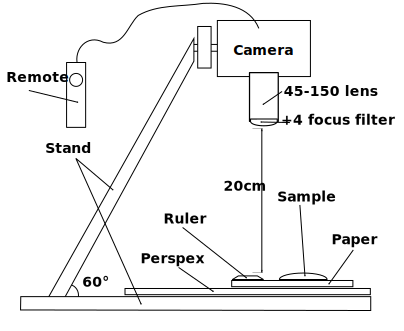
\includegraphics[width=0.5\textwidth]{illustrations/photography_setup.pdf}
  \caption{The setup for photography. A LUMIX G VARIO is used with a
    45-150 zoom lens, placed about 20cm away from the sample.}
  \label{fig:image-setup}
\end{figure}

Pictures are taken using the Lumix G Vario camera with 45-150mm lens
and attached +4 close focus filter (see
Figure~\ref{fig:image-setup}). The camera is set up on a stand mount
to be directly above the sample, at a height of approximately 20cm. A
perspex sheet is placed on top of the stand to make it easier to move
the sample underneath the camera. A remote trigger is used to reduce
camera shake. Ambient diffuse fluorescent lighting is used to provide
light to the sample.

The sample is mounted horizontally on blue seed germination
paper\footnote{Anchor Paper, 19''x24'' Blue Blotter Paper, cut into
  A5-sized sheets}, and a ruler is placed beneath the sample for
scale. The camera is set to minimum zoom, or alternatively the highest
zoom that still allows focusing (check by listening for the beep when
half-pressing the camera shutter button). Because a remote trigger is
used to prevent camera shake, a good image can be produced with ISO
can be set to as low as possible (ISO 160), with shutter speed and
aperture automatically controlled.

\section{Stitching Images}

\begin{figure}
  \centering
  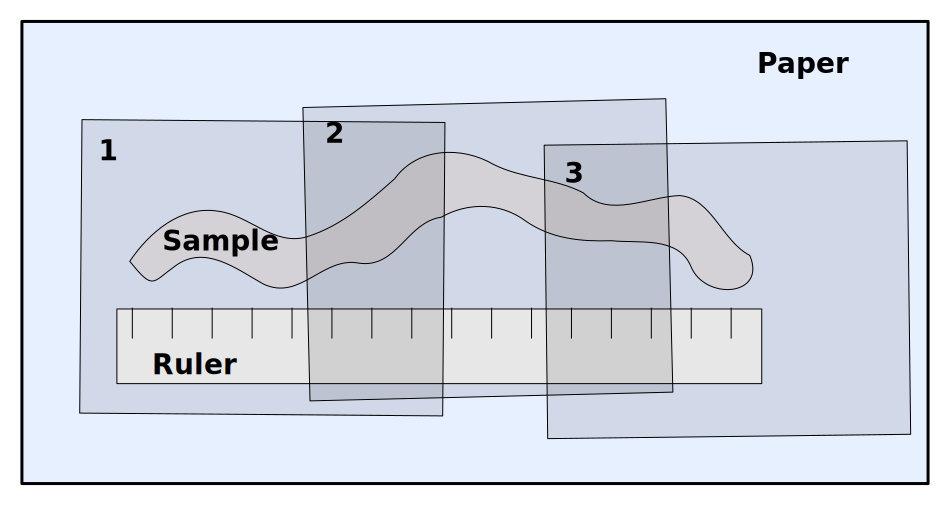
\includegraphics[width=0.5\textwidth]{illustrations/stitching_setup.pdf}
  \caption{Images are easier to stitch using Hugin when laid out
    horizontally. The sample is shifted from right to left underneath
    a fixed camera.}
  \label{fig:stitch-setup}
\end{figure}


When taking images, the stitching process is made simpler by laying
out the sample horizontally, and shifting the paper, sample and ruler
horizontally from right to left (fixed camera, moving sample). Images
should overlap by about 30\% so that matching points can be easily
found on adjacent images. Small changes in vertical position and/or
small rotations should not make the stitching more difficult (see
Figure~\ref{fig:stitch-setup}).

Stitching is carried out using
\href{http://hugin.sourceforge.net/}{Hugin}. While this program is
primarily designed for stitching photos taken from a fixed point
(where the camera is kept in the same place and rotated to cover the
subject), it has translation options that allow it to work effectively
with shifted images.

If there are errors in the stitching process, it may be necessary to
remove control points from the ruler and stitch based on the sample
alone -- Hugin can get a bit confused when it sees too many points
that look the same.

\section{Automatic Scale Calculation}
\label{sec:scale-calc}


An ImageJ macro has been written to automatically detect a [white]
ruler in the image, and calculate a scale. The image is pre-processed
by thresholding at 192/255, so that only extreme black/white colour
changes are preserved. The process works by creating a line that is
one third the image width and sliding it down the centre of the image
at intervals of $\sfrac{1}{40}~height$. Once it detects at least 15
dark regions at regular intervals ($CV < 10\%$) along this line
profile, it works out the pixel distance between the first and last
region, then divides that by the number of regions to get the image
resolution in $\sfrac{px}{mm}$. The scale calculator can handle small
changes in the rotation of the ruler on the image, and rotates the
profile line appropriately:

\begin{Verbatim}
function findMaxima(xx, tolerance){
  // based on "official" findMaxima function from ImageJ 1.48c+
  len = xx.length;
  if (len == 0) {
    return newArray();
  }
  if (tolerance < 0) {
    tolerance = 0;
  }
  maxPositions = Array.copy(xx);
  Array.fill(maxPositions,-1);
  max = xx[0];
  min = xx[0];
  maxPos = 0;
  lastMaxPos = -1;
  leftValleyFound = false;
  maxCount = 0;
  for (jj = 1; jj < len; jj++) {
    val = xx[jj];
    if (val > min + tolerance)
      leftValleyFound = true;
    if (val > max && leftValleyFound) {
      max = val;
      maxPos = jj;
    }
    if (leftValleyFound)
      lastMaxPos = maxPos;
    if (val < max - tolerance && leftValleyFound) {
      maxPositions[maxCount] = maxPos;
      maxCount++;
      leftValleyFound = false;
      min = val;
      max = val;
    }
    if (val < min) {
      min = val;
      if (!leftValleyFound)
	max = val;
    }
  }
  return Array.trim(maxPositions,maxCount);
}

requires("1.44i"); // needed for Array.sort

run("Select None");
ht = getHeight();
wd = getWidth();
oldName = getInfo("image.filename");
fName = "dup_" + oldName;
run("Duplicate...", "title=[" + fName + "]");
selectWindow(fName);
run("8-bit");
setAutoThreshold("Default");
setThreshold(0, 192);
setOption("BlackBackground", false);
run("Convert to Mask");
run("Remove Outliers...", "radius=10 threshold=50 which=Bright");
found = false;
// Calculate image rotation using vertical profile
makeRectangle(wd/3, 10, wd/6, ht-10);
setKeyDown("alt");
p1 = getProfile();
setKeyDown("none");
makeRectangle(wd/3+wd/6, 10, wd/6, ht-10);
setKeyDown("alt");
p2 = getProfile();
setKeyDown("none");
startGr =  p1[floor(p1.length/100)] > p1[(p1.length-1) - floor(p1.length/100)];
ep1 = -1;
ep2 = -1;
for(i = 0; i < p1.length; i++){
      edgeValue = 160; // point where ruler edge should be
      if((ep1 == -1) && ((startGr && p1[i] < edgeValue) ||
                         (!startGr && p1[i] > edgeValue))){
        ep1 = i;
      }
      if((ep2 == -1) && ((startGr && p2[i] < edgeValue) ||
                         (!startGr && p2[i] > edgeValue))){
        ep2 = i;
      }
}
ep1 += 10;
ep2 += 10;
rulerSlope = 0;
if((ep1 != -1) && (ep2 != -1)){
  rulerSlope = (ep2 - ep1) / (wd / 6);
  makeLine(wd/3+wd/12,ep1,wd/3+wd/6+wd/12,ep2);
}
// Calculate scale using line profile
for(i = 0; i < ht; i+= ht/40){
  deviation = wd/6 * rulerSlope;
  makeLine(wd/2-wd/6, i+ht/20-deviation, wd/2+wd/6, i+ht/20+deviation);
  profile = getProfile();
  minLocs = findMaxima(profile, 10);
  Array.sort(minLocs);
  diffs = Array.copy(minLocs);
  if(minLocs.length > 1){
    for(j = 0; j < (minLocs.length-1); j++){
      diffs[j] = minLocs[j+1] - minLocs[j];
    }
    diffs = Array.trim(diffs,minLocs.length-1);
    Array.sort(diffs);
    Array.getStatistics(diffs,min,max,mean,std);
    med = diffs[diffs.length/2];
    cv = abs(std / mean);
    if((cv < 0.1) && (diffs.length > 15)){
      selectWindow(oldName);
      makeLine(minLocs[0]+wd/2-wd/6, i+ht/20-deviation,
              (minLocs[minLocs.length-1]-minLocs[0])+wd/2-wd/6,
               i+ht/20+deviation);
      run("Set Scale...", "distance="+(minLocs[minLocs.length-1]-minLocs[0])+
        " known="+diffs.length+" pixel=1 unit=mm");
      selectWindow(fName);
      found = true;
      i += ht; // end outer loop
    }
  }
}
close();
if(!found){
  exit("Error: Cannot determine scale, ruler could not be found. " +
    "Are you using a colour image with a horizontal white ruler?");
}
\end{Verbatim}

\section{Background Subtraction}

\begin{figure}
  \centering
  \includegraphics[width=0.9\textwidth]{illustrations/small_DkrPaint.jpg}
  \caption{An image of a normal sample that has been stitched using
    Hugin. The region identified as containing a ruler section for
    calculating the scale (see Section~\ref{sec:scale-calc}) has been
    inverted in this image.}
  \label{fig:stitched-image}
\end{figure}

After the image is taken and stitched (see
Figure~\ref{fig:stitched-image}), the background is removed from the
image. By using a blue background, the amount of useful information
that is removed in the background subtraction process is substantially
reduced. The process of background subtraction is carried out in
ImageJ as follows:

\begin{enumerate}
\item Split the image into Red, Green, and Blue channels
\item Normalise each channel to reduce colour split effects
\item combine and Z-project the Red and Green channels using average intensity [optional]
\item Use the Image Calculator to subtract the Blue channel from
  either the Red channel or the combined Red+Green channel
\end{enumerate}

A short ImageJ macro has been written to carry out this background
subtraction process on an arbitrary image. The result of this proces
on Figure~\ref{fig:stitched-image} can be seen in
Figure~\ref{fig:bg-subtract}:

\begin{Verbatim}
// subtract the blue channel from an image
run("Select None");
oldName = getInfo("image.filename");
fName = "dup_" + oldName;
run("Duplicate...", "title=[" + fName + "]");
selectWindow(fName);
run("Split Channels");
selectWindow(fName + " (green)");
close();
selectWindow(fName + " (red)");
run("Enhance Contrast...", "saturated=0 normalize equalize");
selectWindow(fName + " (blue)");
run("Enhance Contrast...", "saturated=0 normalize equalize");
imageCalculator("Subtract create", fName + " (red)",fName + " (blue)");
selectWindow(fName + " (red)");
close();
selectWindow(fName + " (blue)");
close();
selectWindow("Result of " + fName + " (red)");
rename("R-B_" + oldName);
\end{Verbatim}

\begin{figure}
  \centering
  \includegraphics[width=0.9\textwidth]{illustrations/small_R-B_DkrPaint.jpg}
  \caption{A sample with blue background subtracted from the image}
  \label{fig:bg-subtract}
\end{figure}

\section{Feature Extraction}

\begin{figure}
  \centering
  \includegraphics[width=0.9\textwidth]{illustrations/small_foundRegions_DkrPaint.jpg}
  \caption{A sample with tumor-like regions identified by a feature extraction macro}
  \label{fig:feature-extract}
\end{figure}

An ImageJ macro has been written to extract features from a
background-subtracted image that look similar to tumours. The
extraction process is roughly the following:

\begin{enumerate}
\item Threshold the image to black/white
\item Despeckle to remove noisy areas
\item Remove dark outliers (larger noisy bits outside blobs)
\item Remove light outliers (light areas inside blobs, e.g. bubbles,
  light reflections)
\item Apply a watershed filter to separate joined blobs
\item Select remaining regions, then measure those regions on the
  original background-subtracted image
\end{enumerate}

Results relating to the shape and appearance of the features are
stored in the ImageJ results table. The features are outlined and
transferred back to the original (non-subtracted) image as an overlay.

The result of this process on Figure~\ref{fig:stitched-image} can be
seen in Figure~\ref{fig:feature-extract}. Note that this was a normal
sample, but tumour-like features were detected in it.

\begin{Verbatim}
  oldName = getInfo("image.filename");

  if(!is("grayscale")){
    // background subtraction hasn't been carried out first, so do that
    run("Autoscale");
    run("SubtractBlue");
  } else {
    oldName = replace(oldName,"^R-B_","");
  }

  getPixelSize(unit, pw, ph, pd);
  if(unit != "mm"){
    exit("Error: scale is not in millimetres (mm). " +
    "Has the scale been set?");
  }

  selectWindow("R-B_" + oldName);
  greyName = "grey_" + oldName;
  run("Duplicate...", "title=[" + greyName + "]");

  selectWindow("R-B_" + oldName);
  setAutoThreshold("Default bright");
  setOption("BlackBackground", false);
  run("Convert to Mask");
  run("Invert");
  run("Despeckle");
  run("Remove Outliers...", "radius=25 threshold=50 which=Dark");
  run("Remove Outliers...", "radius=25 threshold=50 which=Bright");
  run("Watershed");
  run("Set Measurements...", "area mean standard modal min centroid "+
        "center perimeter bounding fit shape feret's integrated median "+
        "skewness kurtosis area_fraction redirect=None decimal=3");
  run("Analyze Particles...", "size=0.20-Infinity circularity=0-1.00 "+
        "show=[Overlay Outlines] display exclude clear");
  if(Overlay.size > 0){
    Overlay.copy();
    close("R-B_" + oldName);
    selectWindow(oldName);
    Overlay.paste();
    // re-analyse particle regions using greyscale image
    selectWindow(greyName);
    Overlay.paste();
    run("To ROI Manager");
    run("Clear Results");
    roiManager("Measure");
    selectWindow("ROI Manager");
    run("Close");
    close(greyName);
    selectWindow("Results");
  } else { // no overlay, so don't try to copy it
    close("R-B_" + oldName);
    selectWindow(oldName);
  }
\end{Verbatim}

\section{Statistical Analysis}

\emph{This section has yet to be written / carried out. It will
  probably involve an R script that processes measurement data from
  the Feature Extraction step.}

\end{document}
